\chapter{Formáty uložení řídkých matic}

Formáty uložení řídkých matic obecně ukládají jednotlivé elementy zvlášť a tedy nemusí ukládat ty nulové. To ale přináší řadu nevýhod. Za prvé se musí ukládat informace o souřadicních jednotliých prvcích. Za druhé, ztrácíme možnost přístupu k prvku na libovolných šouřadnicích v čase $\Theta(1)$, protože prvky nemáme přímo indexované podle jejich umístění v řádku a sloupci.

Protože řídké matice můžeme rozdělit do mnoha kategorií a provádět nad nimi mnoho operací, existuje hodně formátů, jak řídkou matici efektivně uložit a pracovat s ní.

\subsection{Modifikace řídké matice}

Formáty uložení řídkých matic můžeme také rozdělit podle toho, zda-li je možné do nich přidávat nebo odebírat prvky.

Při násobení matic $C = A \cdot B$ se matice $A$ ani $B$ nemění. V této práci budeme předpokládat, že matice $C$ bude hustá a formáty umožujícími přidávání nebo odebírání prvků nebudou součástí práce. Stejně tak při násobení matice $A$ vektorem $B$ je výsledek $C$ vektor.

\subsection{Uspořádanost řídké matice}

Dalším kritériem pro rozdělení formátů je uspořádanost nenulových prvků v řídké matici. Pro uspořádané prvky bude efektivnější takový formát, který využije určitý vzor. V řídkých maticích takovým vzorem může být například diagonála, nebo blok prvků. Efektivně lze za vzor považovat i prvky v řádku, nebo ve sloupci.

Uspořádáním může být také symetrie matice, kdy nám stačí uložit pouze polovinu matice. Zpravidla řídké matice bývají symetrické podle hlavní diagonály.

\section{COO - Coordinate list}

Formát COO, česky seznam souřadnic, je základní formát řídkých matic. Ke~každému nenulovému prvku ukládá jeho souřadnice \texttt{y} a \texttt{x}. Implementovat tento formát můžeme například jako tři pole, jedno s hodnotami prvků, druhé s \texttt{y} souřadnicemi a třetí s \texttt{x} souřadnicemi.

Pro ukázku v tomto formátu uložíme matici o velikosti $n=8$ s $nnz=5$ nenulovými prvky.

\begin{align}
\begin{pmatrix}
	0 & 0 & 0 & 0 & 0 & 0 & 0 & 0 \\
	\boldsymbol{1} & \boldsymbol{2} & 0 & 0 & 0 & 0 & 0 & 0 \\
	0 & 0 & 0 & 0 & 0 & 0 & 0 & 0 \\
	0 & 0 & 0 & 0 & 0 & 0 & 0 & 0 \\
	0 & \boldsymbol{3} & 0 & 0 & 0 & 0 & 0 & 0 \\
	0 & 0 & 0 & 0 & 0 & 0 & 0 & 0 \\
	0 & 0 & 0 & 0 & 0 & \boldsymbol{4} & \boldsymbol{5} & 0 \\
	0 & 0 & 0 & 0 & 0 & 0 & 0 & 0 \\	
\end{pmatrix}
\end{align}

\begin{table}[H]
    \begin{tabular}{r|lllll}
    values[5]   & 1 & 2 & 3 & 4 & 5 \\
    y-coords[5] & 1 & 1 & 4 & 7 & 7 \\
    x-coords[5] & 0 & 1 & 1 & 5 & 6 \\
    \end{tabular}
    \caption{Matice uložená ve formátu COO}
\end{table}

Jak můžeme vidět, délka polí je závislá pouze na $nnz$. Pro velké matice s malým počtem neuspořádaných nenulových prvků je tento formát velmi efektivní. Pokud by bylo prvků velké množství, informace o uložení \texttt{y} nebo \texttt{x} souřadnic by byla často redundatní.

\section{CSR - Compressed sparse row}

Problém efektivnosti formátu COO pro větší množství prvků řeší formát CSR, česky řádky komprimovaných vektorů. Formát CSR obsahuje pole $row\_pointers$, které obsahuje informaci o tom, kolik se v daném řádku nachází prvků. K poli s hodnotami je další pole $col\_indicies$, přiřazující ke každému prvku informaci o sloupci.

\begin{figure}[H]\centering
	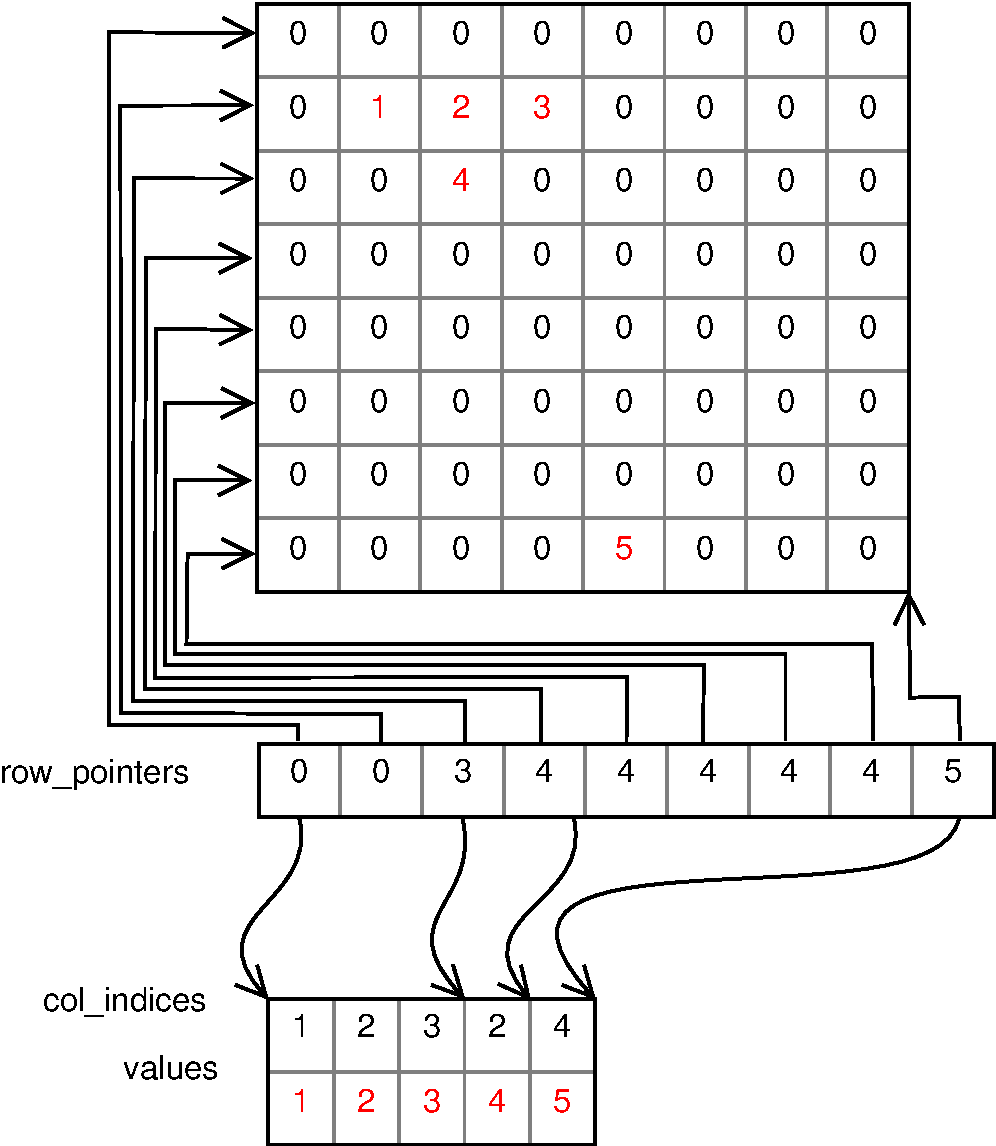
\includegraphics[width=\textwidth]{./images/csr/csr}
	\caption{Matice uložená ve formátu CSR}
	\label{fig:CSR}
\end{figure}

\section{BSR - Block Sparse Row}

\url{https://software.intel.com/sites/products/documentation/doclib/mkl_sa/11/mklman/GUID-9FCEB1C4-670D-4738-81D2-F378013412B0.htm}



\section{Quadtree}

\section{?}

TODO: tady jsem chtel spocictat kdy  se vyplati mit ridkou matici, ale lepsi bude tabulka. Pokud například uložíme matici o rozměrech 100x100 v dvojté přestnosti, bude zabírat \texttt{M x N x sizeof(double) = 100 x 100 x 8 = 80000B = 80kB}. Pokud zvolíme řídký formát matice, kde ke každému elementu uložíme i jeho x a y souřadnici, tak do 80kB uložíme \texttt{80000 / (sizeof(int)+sizeof(int)+sizeof(double)) = 80000/16= 5000} elementů. Pokud matice obsahuje více jak 50  \% nulových elementů, vyplatí se nám ji uložit do řídkého formátu.

%-----------------------------------------------------------------------------

\chapter{Modifikace formátu quadtree}

je to samostatnej bod v zadani tak by to mohla byt cela chapter

TODO: popsat nevyhody quadtree a obrazkama ukazat jak to udelat lip

neco jako quadtree loop unrolling
